\chapter{Results}\label{ch:results}

Please note: this chapter is written as a demonstrator section for expediency. The original plan was to draw out from the interviews mentions pertaining to each factor in the ISM framework. However, this is proving to be a huge undertaking. Instead, I propose to only work with a few of the factors that are relevant to scientists' roles. For instance, these may be Values, beliefs, attitudes, (currently unfinished Section~\ref{sec:resismvalues}), Opinion leaders (currently slightly more finished Section~\ref{sec:resopinionleaders}) and Roles and identity (currently slightly more finished Section~\ref{sec:resroles}). This may be plenty if I include the discussion that ties these three elements together with published work on roles at the science policy interface. 

Where relevant below, I explain the current state of the chapter. Section~\ref{sec:resindividual}, the chapter on individual factors that influence behaviour, has not been updated from the first test run, because I have not had time - and now I wonder if most of it will be removed. Instead, I have focused more attention on Section~\ref{sec:ressocial}, the social factors that influence behaviours, because this appears to be more important to participants (based on the number of stories that mention these factors). I process the two social factors (Opinion leaders and Roles and identity) that I suggest above.

Quick summary - because there is no methods section. Within the interviews, chunks of description pertaining to the same theme were grouped into ``stories''. This was a more logical unit than sentence or participant. Each of these stories comprised multiple statements and each statement was labelled according to how it referenced one or more of 18 different factors that influence behaviour, as described in the ISM framework. I labelled on those factors that influenced the behaviour of scientists, but some of them may appear to be more to do with others (such as a policymaker requiring a \emph{skill} in CAN science, which affects how well a scientist can engage with them).

A total of 155 stories\improvement{make sure stories are explained in Chapter~\ref{ch:methods}} were identified in the interviews, excluding those pertaining to the participants' introductory statements about their field of work. Frequently, a story would contain multiple labels for the same theme. For instance, Story 45 ``frustrations as a scientist compared to those as a concerned citizen'' contained mentions of 3 different roles, as well as a description of a conflict in roles. Section~\ref{sec:resultsISM} discusses the nature of each of the ISM factors as they surface within the interviews.

\section{Drivers and barriers to CAN science-policy engagement}\label{sec:resultsISM}

\begin{figure}[!ht]
    \centering
    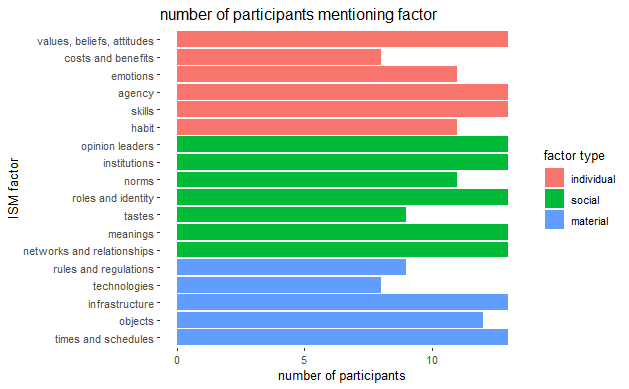
\includegraphics[width=1\linewidth]{figures/participants_mentioning_ism_factor.png}
    \caption{Number of participants mentioning ISM factors}
    \label{fig:ismparticipantcount}
\end{figure}

\begin{figure}[!ht]
    \centering
    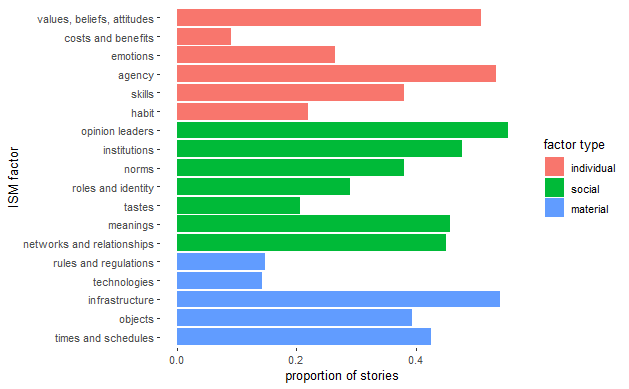
\includegraphics[width=1\linewidth]{figures/stories_mentioning_ism_factor.png}
    \caption{Number of stories mentioning ISM factors}
    \label{fig:ismstorycount}
\end{figure}

\begin{figure}[!ht]
    \centering
    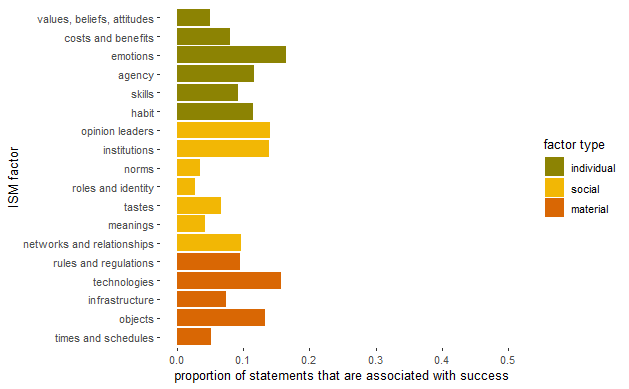
\includegraphics[width=1\linewidth]{figures/statements_associated_with_success.png}
    \caption{Proportion of statements for each ISM factor that are associated with success}
    \label{fig:ismsuccess}
\end{figure}

\begin{figure}[!ht]
    \centering
    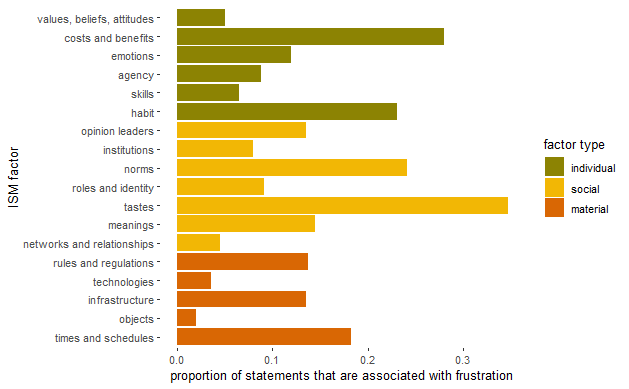
\includegraphics[width=1\linewidth]{figures/statements_associated_with_frustration.png}
    \caption{Proportion of statements for each ISM factor that are associated with frustration}
    \label{fig:ismfrustration}
\end{figure}

%\begin{figure}[!ht]
%    \centering
%    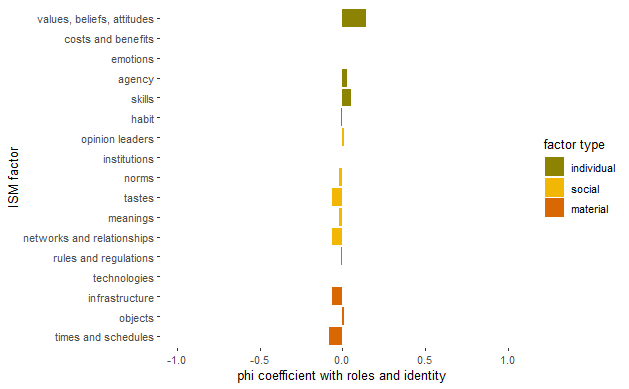
\includegraphics[width=1\linewidth]{figures/phi_coefficient_with_rolesandidentity.png}
%    \caption{Phi coefficient for each ISM factor against \ismsr}
%    \label{fig:ismphiroles}
%\end{figure}

%\begin{figure}[!ht]
%    \centering
%    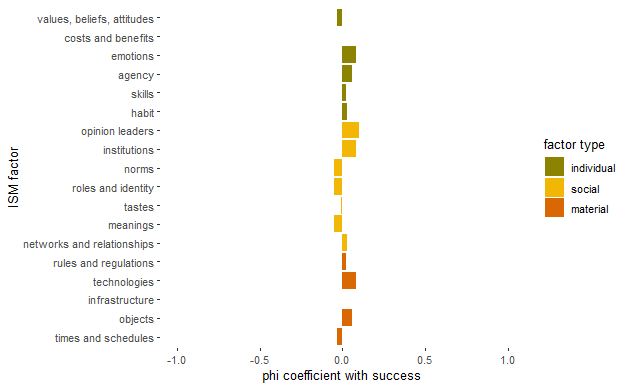
\includegraphics[width=1\linewidth]{figures/phi_coefficient_with_success.png}
%    \caption{Phi coefficient for each ISM factor against success}
%    \label{fig:ismphisuccess}
%\end{figure}

%\begin{figure}[!ht]
%    \centering
%    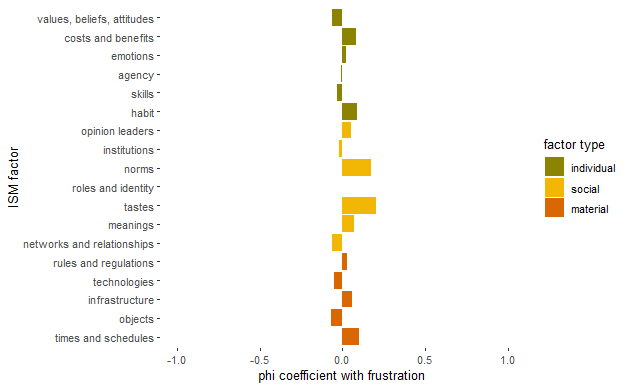
\includegraphics[width=1\linewidth]{figures/phi_coefficient_with_frustration.png}
%    \caption{Phi coefficient for each ISM factor against frustration}
%    \label{fig:ismphifrustration}
%\end{figure}

The ISM framework\improvement{make sure this is explained and referenced in Chapter~\ref{ch:lit} and how I used it is described in Chapter~\ref{ch:methods}} was used to identify the behaviour factors that enable or inhibit engagement and influence at the science policy interface. Figure~\ref{fig:ismstorycount} shows the number of stories in which each factor was mentioned. Each section below describes the nature of the drivers for each of 18 behavioural factors, as identified in the interviews.

Each the ISM factor was mentioned by at least half the participants.

\subsection{Individual factors}\label{sec:resindividual}

A wide range of factors relating to the individual participants' motivation were identified in the interviews. All participants identified \ismiv, \ismia{} and \ismis.  \ismiv{} and \ismia{} appeared in more than half the stories. \ismic{} was the least mentioned of all the ISM factors. Both \ismis{} and \ismih{} included observations the influences that the \ismis{} and \ismih{} of others had the quality of engagement.

\subsubsection{\ismiv}\label{sec:resismvalues}

\begin{table}[!ht]
\footnotesize
\caption{The main examples of \ismiv{} that influences CAN science and policy  engagements found in the interviews and example quotes}\label{tab:resvalues}
\begin{tabular}{L{.06\linewidth}L{.3\linewidth}L{.12\linewidth}L{.52\linewidth}} \hline
\textbf{id} & \textbf{\ismiv} & \textbf{influence} & \textbf{example quote} \\ \hline \hline 
iv1 & duty to try & enabling & \tquote{it's better to try than not try}{p03}{143} \\[5mm]
iv2 & moral imperative & enabling & \tquote{it would be morally not possible to not want to do the engagement if you knew the things I found out}{p08}{131} \\[5mm]
iv3 & social justice & enabling & \tquote{with very strongly held contested views on both sides of the debate ... it's actually rewarding in that often you can help to find a common ground}{p13}{68} \\[5mm]
iv4 & science should be useful (in general) & enabling & \tquote{when we're writing papers now, we want to make sure that they're going to be useful to to policy makers}{p02}{64} \\[5mm]
iv5 & science should be relevant & various & \tquote{in that programme we were thinking about the science but we tailored the questions that we asked so that they would have policy relevance}{p13}{15} \\[5mm]
%iv8 &  & inhibiting & \tquote{I look around madly, how can I get technology into my research so I can get it funded? I need technology ... because if I don't, I don't have any relevance}{p11}{70} \\[5mm]
iv6 & science should be credible & neutral & \tquote{I very much had to ground myself in what the science was saying and not say the UK government isn't doing enough}{p04}{29} \\[5mm]
iv7 & science should be open & neutral & \tquote{I've always really felt it important to make sure that the science that we do, that people know about it, that it doesn't just end up in an academic paper}{p14}{5} \\[5mm]
iv8 & science should be responsible & neutral & \tquote{you need to do the work and do as you start doing it, think about the environmental and societal impacts of it}{p01}{109} \\[5mm]
iv9 & we should challenge current policy approaches & neutral & \tquote{everyone would have some doubts about the strength of the pure cost benefit analysis approach to a climate problem}{p08}{95} \\[5mm]
iv10 & it is important to share what I know & enabling & \tquote{I have a few key messages and I want to try to do something with them}{p05}{102} \\[5mm]
iv11 & policy should be based on the best science & enabling & \tquote{one of the best ways that you can actually have long term impact on policy is by doing the the fundamental science that is going to be needed to inform long term policy decisions}{p13}{18} \\[5mm]
iv12 & we should be pragmatic & various & \tquote{lobbying sounds like a dirty word, but we're lobbying based on the best available science}{p06}{92} \\[5mm]
iv13 & value for public money & neutral & \tquote{this is mostly taxpayers money, it should be useful}{p07}{48} \\[5mm] \hline
\end{tabular}
\end{table}


Participants stated a range of \ismiv{} that motivated them to undertake policy-relevant science and engage with policy, such as a values relating to duty (iv1), moral imperative (iv2), and social justice (iv3). Many participants expressed beliefs about their science, such as that it should be useful (iv4), relevant (iv5), credible (iv6), open (iv7) and responsible (iv8). Engagements with policy were often driven by a belief that it is important to share knowledge (iv10) and that policy should be based on the best science (iv11). Finally, participants also acknowledge some attitudes to their work about being pragmatic (iv12) and returning value for public money.

\paragraph{Strategies:}
Because, in most cases, \ismiv{} had an enabling or neutral influence on engagements, strategies related to them tended to be to align to those values, beliefs or attitudes, and these therefore have not been further tabulated in this section. For instance, \tref{a participant who felt strongly that science should be credible}{p09} used a strategy \tquote{not to mislead, willingly or unwillingly}{p09}{74}.

\subsubsection{\ismic}\label{sec:resismcab}

\begin{table}[!ht]
\footnotesize
\caption{The main examples of expressions of \ismic{} that influences CAN science and policy engagements found in the interviews and example quotes}\label{tab:rescosts}
\begin{tabular}{L{.06\linewidth}L{.3\linewidth}L{.12\linewidth}L{.52\linewidth}} \hline
\textbf{id} & \textbf{\ismic} & \textbf{influence} & \textbf{example quote} \\ \hline \hline 
icb1 & too much effort & inhibiting & \tquote{life's too short and there's too much hard work to do on the research, to spend too much of your time [strategically targeting policymakers]}{p08}{50} \\[5mm]
icb2 & is the effort worth it? & various & \tquote{governments have enough information on which to act already and have quite sufficient evidence}{p04}{48} \\[5mm]
icb3 & its worth it & enabling & \tquote{If it's going to be useful, why wouldn't we prioritise our time to do that paper rather than something else}{p01}{78} \\[5mm] \hline
\end{tabular}
\end{table}

A weighing up of \ismic{} didn't feature a great deal in the interviews. Where it did, it tended to be about the effort it takes to engage with policy, against the worth of the outcomes. These range from feeling some aspects of engagement were too much effort (icb1), or worth the effort (icb3), or questioning whether the effort is worthwhile (icb2). Most participants stating only one position, \tref{although one participant stated all three positions}{p08}. 

\begin{table}[!ht]
\footnotesize
\caption{The strategies related to \ismic{} found in the interviews and example quotes}\label{tab:rescostsstrat}
\begin{tabular}{L{.06\linewidth}L{.3\linewidth}L{.64\linewidth}} \hline
\textbf{id} & \textbf{strategy} & \textbf{example quote} \\ \hline \hline
icbs1 & spreading the opportunities for success & \tquote{policy can be super powerful and continue perhaps to put the prime emphasis on those actors, but wouldn't put all my eggs in that basket}{p08}{144} \\[5mm] \hline
 \end{tabular}
\end{table}

\paragraph{Strategies:}
Two participants had strategies that spread opportunities for success (icbs1), which tended to involve engaging with a range of actors, not just those directly making policy decisions.

%There was very little indication of scientists weighing up the costs and benefits of their work or that of others. One scientist balanced the value of their activity with its used for policymaking and concluded that \emph{it's worth it} - \tquote{If it's going to be useful, why wouldn't we prioritise our time to do that paper rather than something else}{p01}{}, this was linked to an acknowledgement of the costs and benefits to policymakers for whom reading all the relevant scientific literature is \emph{too much effort}. Regarding engaging at the science policy interface, another scientist felt that they were \emph{not sure its worth the effort} - \tquote{I'm not convinced that it overall is hugely impactful}{p03}{}

\subsubsection{\ismie}\label{sec:resismemotions}

\begin{table}[!ht]
\footnotesize
\caption{The main examples of \ismie{} that influences CAN science and policy  engagements found in the interviews and example quotes}\label{tab:res****}
\begin{tabular}{L{.06\linewidth}L{.3\linewidth}L{.12\linewidth}L{.52\linewidth}} \hline
\textbf{id} & \textbf{\ismie} & \textbf{influence} & \textbf{example quote} \\ \hline \hline 
ie1 & curiosity; gratitude; pride; satisfaction; determination & enabling & \tquote{it is ultimately rewarding to get involved in some of the really knotty challenges where there's a lot of controversy}{p13}{67} \vfill \tquote{I'm proud of it because it was a beautiful thing that we created and a process that was really interesting
}{p05}{108} \\[5mm] 
ie2 & surprise; disappointment; despair; frustration; exhaustion & inhibiting & \tquote{I'm just kind of disappointed that with policy … in the UK, we get there but its very, very complex}{p08}{72} \vfill \tquote{I look around me and I see the promises of 20-30 years just gone}{p11}{84} \\[5mm] \hline
\end{tabular}
\end{table}

Various \ismie{} were associated with undertaking science and engaging with policy, often as a response to the experiences. Some of these were positive experiences and often provided motivation to continue with engagements (ie1). Other were experienced as demotivators and inhibitors (ie2).

\paragraph{Strategies:}
Because \ismie{} tended to be experience in response to experiences related to policy engagements, there were no strategies given to directly address the experience of emotions. However, strategic actions (related to other ISM factors) could result in experiences of pride and satisfaction.

\subsubsection{\ismia}\label{sec:resismagency}

\begin{table}[!ht]
\footnotesize
\caption{The main examples of \ismia{} that influences CAN science and policy  engagements found in the interviews and example quotes}\label{tab:resagency}
\begin{tabular}{L{.06\linewidth}L{.3\linewidth}L{.12\linewidth}L{.52\linewidth}} \hline
\textbf{id} & \textbf{\ismia} & \textbf{influence} & \textbf{example quote} \\ \hline \hline 
ia1 & having capability & enabling & \tquote{we're certainly getting them thinking}{p08}{90} \\[5mm]
ia2 & happenstance & various & \tquote{really so much of the policy process is about being in the right place at the right time}{p10}{55} \\[5mm]
ia3 & limits to my influence & inhibiting & \tquote{I don't know whether I can really claim that my specific research has impacted}{p12}{39} \\[5mm] \hline
\end{tabular}
\end{table}

\ismia{} was the most commonly expressed individual influence in terms of stories. This influence could be enabling, with participants expressing how they have confidence in their ability (ia1), inhibiting, where participants identified that their influence is limited (ia3), or they identified the influence of chance on a number of aspects of their work, particularly the ability to engage with policy (ris2).

\begin{table}[!ht]
\footnotesize
\caption{The strategies related to \ismia{} found in the interviews and example quotes}\label{tab:resagencystrat}
\begin{tabular}{L{.06\linewidth}L{.3\linewidth}L{.64\linewidth}} \hline
\textbf{id} & \textbf{strategy} & \textbf{example quote} \\ \hline \hline
ias1 & making it happen & \tquote{making sure that when policy windows or relationships emerge, that you can leverage them or you can use them to influence policy}{p12}{83} \\[5mm] \hline
 \end{tabular}
\end{table}

\paragraph{Strategies:}
Given the influence of chance the initiation and outcomes of engagements with policy, a number of participants identified that they tried to be ready for openings for engagement (ias1), which relates to building knowledge in the policymaking process (Section~\ref{sec:resismskills}) and anticipating changes in policy (Section~\ref{sec:resrules}).

\subsubsection{\ismis}\label{sec:resismskills}

\begin{table}[!ht]
\footnotesize
\caption{The main examples of observations related to \ismis{} that influences CAN science and policy  engagements found in the interviews and example quotes}\label{tab:res****}
\begin{tabular}{L{.06\linewidth}L{.3\linewidth}L{.12\linewidth}L{.52\linewidth}} \hline
\textbf{id} & \textbf{observation} & \textbf{influence} & \textbf{example quote} \\ \hline \hline 
is1 & I know and understand the science & enabling & \tquote{actually we're probably the best people to be speaking to}{p01}{43} \\[5mm]
is2 & I know and understand the policymaking process & enabling & \tquote{because we've been speaking to some of the policy people as part of that, we knew this is just setting the policy landscape}{p01}{86} \\[5mm]
%is3 & the policymaker knows and understands the area of policy & enabling & \tquote{what are we going to do when [policy official] goes, he's the glue. All of these fresh, young things that constantly appear and move on and move on, there's very few of those stable kind of people with that legacy knowledge of what we did last time or how things were before}{p14}{108} \\[5mm]
is3 & the policymaker can gain knowledge easily & enabling & \tquote{there is a receptivity to that argument, particularly amongst the bright people in the civil service - they totally get that}{p08}{107} \\[5mm]
is4 & I need to gain knowledge in the science & neutral & \tquote{I do need to be in touch with colleagues and coming into the office and stay in contact with them and ask some questions about things to try and draw out what it is that might be of interest}{p07}{35} \\[5mm]
is5 & I need to gain knowledge in the policymaking process & inhibiting & \tquote{it felt like we were worlds apart in terms of what we could provide and what they really needed and also the language that they speak was very different to ours}{p04}{61} \\[5mm]
is6 & the policymaker needs to gain knowledge in the science & inhibiting & \tquote{I realised there's a huge challenge there in terms of just understanding each other's domain, so that we understand what they need and we and likewise they can understand the limits of what we can provide}{p04}{61} \\[5mm]
 \hline
\end{tabular}
\end{table}

\ismis{} was interpreted as being largely about knowledge, both of CAN science and of policymaking processes. These were influential because lack of the right knowledge made engagement considerably harder. In particular, participants understand the relevant science (is1) or policymaking process (is2) was, understandably, beneficial to engagement, as was working with policy people who cold gain new knowledge easily (is3). Where participants expressed that they need to gain scientific knowledge (is5), this wasn't seen has inhibiting, simply part of their role. However, barriers to engagement were noted when the participant felt they needed to understand the policymaking process better (is5) or when working with policymakers who needed to gain more knowledge about relevant science (is6). 

\begin{table}[!ht]
\footnotesize
\caption{The strategies related to \ismis{} found in the interviews and example quotes}\label{tab:resskillsstrat}
\begin{tabular}{L{.06\linewidth}L{.3\linewidth}L{.64\linewidth}} \hline
\textbf{id} & \textbf{strategy} & \textbf{example quote} \\ \hline \hline
iss1 & working together to build knowledge & \tquote{We scoped out the research with them - they had a quite a clear idea about what they wanted to achieve}{p05}{27} \\[5mm] \hline
 \end{tabular}
\end{table}

\paragraph{Strategies:}
Apart from the very direct strategy of gaining those missing skills, some participants described how they worked together with policymakers to develop the knowledge needed. This is closely related to the strategy of coproduction (Section~\ref{sec:restechnologies}).

\subsubsection{\ismih}\label{sec:resismhabit}

\begin{table}[!ht]
\footnotesize
\caption{The main examples of \ismih{} that influences CAN science and policy  engagements found in the interviews and example quotes}\label{tab:reshabit}
\begin{tabular}{L{.06\linewidth}L{.3\linewidth}L{.12\linewidth}L{.52\linewidth}} \hline
\textbf{id} & \textbf{\ismih} & \textbf{influence} & \textbf{example quote} \\ \hline \hline 
ih1 & scientists doing science for scientists & various & \tquote{you're doing science and you're publishing papers and the people who read those papers are only doing it because they need stuff to cite their study}{p03}{122} \\[5mm]
ih2 & scientists applying the deficit model to create change & various & \tquote{you'd think: give the policymaker the information and they'll act}{p05}{95} \\[5mm]
ih3 & policy obtaining information from the same sources & various & \tquote{I was like, where's the social science in here, you keep bringing in the physical academies and not the social science}{p06}{60} \\[5mm]
ih4 & policymakers using the same policymaking approach & various & \tquote{…they'll just continue to do the same thing and make the same mistakes or have the same assumptions about what works to change behaviour}{p05}{85} \\[5mm]
 \hline
\end{tabular}
\end{table}

\ismih{} was interpreted as behaviours that were particular to either scientists or policymakers that could often go unquestioned - except that they were identified by participants precisely because they were questioning them.  Four main \ismih{} types were identified within the interviews, two being habits of scientists and two of policymakers. Firstly, there can be a tendency for science to be produced only for scientists (ih1). It was also noticed that scientists could habitually use a model of policy change based solely on the idea that not enough information is available to policymakers (ih2). Policymakers were observed going to the same sources for their information and evidence (ih3) as well as using the same approaches (1h4) such as particular economic models.

\begin{table}[!ht]
\footnotesize
\caption{The strategies related to \ismih{} found in the interviews and example quotes}\label{tab:reshabitstrat}
\begin{tabular}{L{.06\linewidth}L{.3\linewidth}L{.64\linewidth}} \hline
\textbf{id} & \textbf{strategy} & \textbf{example quote} \\ \hline \hline
ihs1 & open to new ideas & \tquote{[you're] looking for other ways of tackling things, taking a different perspective on things}{p07}{7} \\[5mm]
\hline
 \end{tabular}
\end{table}

\paragraph{Strategies:}
To break out of habits, participants noted their own, and others', efforts to find new ideas and ways of working (ihs1).
 
\subsection{Social factors}\label{sec:ressocial}


\subsubsection{Opinion leaders}\label{sec:resopinionleaders}

\begin{table}[!ht]
\footnotesize
\caption{The 7 types of mention of \emph{opinion leaders} in the interviews and example quotes for each type}\label{tab:resopinionleaders}
%\begin{tabularx}{\textwidth} {DIQ} 
\begin{tabular}{L{.08\linewidth}L{.3\linewidth}L{.1\linewidth}L{.42\linewidth}}\hline
\textbf{id} & \textbf{observation} & \textbf{influence} & \textbf{example quote} \\ \hline \hline 
ol1 & scientists' knowledge   drew interest from policymakers & enabler & \tquote{They had already decided they wanted to work with us}{p05}{}  \\[5mm]
ol2 & scientists influencing policymakers & enabler & \tquote{Informally I think they [have been] picked up and had a bit of traction}{p03}{}  \\[5mm]
ol3 & scientists influencing others & enabler & \tquote{We've been cited by both industry and NGOs on different sides of the debate, so we've probably got something right there}{p01}{} \\[5mm]
ol4 & senior scientists are more likely to be   listened to & enabler & \tquote{When it comes to something for more formal like that, they tend to go for the professors}{p03}{} \\[5mm]
ol5 & I look up to other scientists & enabler & \tquote{He's an excellent scientist, he's very inclusive and he's   incredibly motivational from a scientific perspective, very much in favour of   community building}{p04}{} \\[5mm]
ol6 & others influence policymakers & inhibitor & \tquote{Sometimes what they bring is politically convenient, and policymaking is not just about evidence is also about political convenience   or political opportunity. They provide narratives to use or discard certain evidence}{p09}{}  \\[5mm]
ol7 & policymakers have influence & neutral & \tquote{I think policy makers have the greatest leverage of   all}{p08}{} \\[5mm] \hline \hline
\textbf{id} & \textbf{strategy} &  \multicolumn{2}{L{.52\linewidth}}{\textbf{example quote}} \\ \hline \hline 
ols1 & opportunities to promote my/our work & \multicolumn{2}{L{.52\linewidth}}{\tquote{If I get media requests, I think if I've got the expertise, I   should do that because it goes with the job}{p01}{}}  \\[5mm]
ols2 &  opportunities to understand the perspectives of policymakers & \multicolumn{2}{L{.52\linewidth}}{\tquote{we try and find out what their priorities are}{p12}{}} \\[5mm] \hline
\end{tabular}
%\end{tabularx}
\end{table}
\improvement{the layout of this table needs to be easier to read}

Nearly half of the stories mention individuals and groups to whom scientists and policymakers will reach out, and be influenced by - more than any other social factor. This indicates that opinion leaders are important to scientists engaging with policy. Given the criteria for inviting people to take part in this study, it is not surprising that many participants mentioned being invited by policymakers to share their knowledge (ol1). Others identified that they believed they had had some influence on policymaking (ol2) or others, such as industry and NGOs (ol3). The was specific recognition that senior scientists are more likely to have influence (ol4).  

It was also quite common to observe that there are non-science actors, such as other governments, industry, learned societies, research councils, special advisers and NGOs, who have influence in the decisions being make (ol6). Further, policymakers themselves were considered to have influence (ol7)

\paragraph{Strategies:}

In some cases, this understanding has been used to gain influence. A number of participants mentioned promoting their work through third parties such as media opportunities but also by engaging with organisations such as industry or NGOs such as charities, campaigning organisations and networks (think tanks) as a mechanism for influencing policymaking (ols1). A different approach was to make efforts to align with policymakers by taking up opportunities to listen to their perspectives (ols2).

\subsubsection{Institutions}\label{sec:resinstitutions}

\begin{table}[!ht]
\footnotesize
\caption{The main influences that \emph{institutions} represented in the interviews and example quotes for each type}\label{tab:resinstitutions}
\begin{tabular}{L{.06\linewidth}L{.32\linewidth}L{.12\linewidth}L{.5\linewidth}} \hline
\textbf{id} & \textbf{observation} & \textbf{influence} & \textbf{example quote} \\ \hline \hline 
i1 & within my institution there is an expectation (to engage with policy; to maintain neutrality; to avoid some topics; to create impact; to write papers; to represent it at events; to write briefings) & various & \tquote{that was very much the culture of that centre was doing work [that] was trying also to impact the world outside academia}{p10}{14} \\[5mm]
i2 & evaluation of our work (by demonstrating impact; by citations; by identifying where we have been influential; by process not outcome; by outputs; by publications) & enabling & \tquote{I've picked up on, certainly from the Research Council … I think all of probably UKRI, policy engagement seems to have the same sort of value as industry engagement}{p01}{103} \\[5mm]
i3 & evaluation of our work (by CAN outcomes; can be ambiguous) & inhibiting & \tquote{having meetings with government departments or sitting on advisory committees, you can't always say `see this piece of advice that has led to this action'}{p05}{23} \\[5mm]
i4 & the evaluation of policy (is very limited; is limited to the obligation to respond; is focused on measureable policy outcomes) & inhibiting & \tquote{they often just don't even evaluate their policies}{p05}{83} \hfill \tquote{the policy makers need measurable things - organisations, to be accountable, need data and statistics}{p11}{33} \\[5mm]
i5 & the evaluation of policy (was possible by giving feedback) & enabling & \tquote{They took every recommendation we had. That was really impactful, albeit in a very tiny area}{p05}{68} \\[5mm]
i6 & policy institutions (have distinct ways of working; are changing slowly; are functioning on limited resources) & various & \tquote{I found the ... hierarchy quite interesting - in a meeting, why is someone else saying what I could just say, why do I have to write the notes so that they can say it ... you have to prepare all these briefings and notes for people to say}{p06}{58} \\[5mm]
i7 & the policy process (has defined timeframes; has defined subject frames; has defined roles) & various & \tquote{you can write the the nicest paper and write the nicest briefing and the nicest translation of that, but people won't listen to you because the decision has been made}{p09}{93} \\[5mm]
i8 & the policy process (is difficult to understand) & inhibiting & \tquote{I think it's often very difficult to know how advice gets used}{p05}{22} \\[5mm]
i9 & we are able to choose our field of research & enabling & \\[5mm]
i10 & we have a social responsibility as a public organisation & neutral & \\[5mm] \hline
\end{tabular}
\end{table}

\begin{table}[!ht]
\footnotesize
\caption{The strategies  \emph{institutions} with example quotes for each}\label{tab:resinstitutionstrat}
\begin{tabular}{L{.06\linewidth}L{.3\linewidth}L{.64\linewidth}} \hline
\textbf{id} & \textbf{strategy} & \textbf{example quote} \\ \hline  \hline
is1 & engage with policy where possible & \tquote{maybe we'll ask them to sit on an Advisory Board}{p12}{7} \\[5mm]
is2 & select policy-related research topics & \tquote{we'd focus on the areas to do with [the biophysical environment], choosing things where we knew that humans might want to interact}{p13}{17} \\[5mm]
is3 & produce evidence that is relevant and timely & \tquote{be aware of the window of opportunity you have to provide evidence that can contribute to the conversation. At some point certain conversation is concluded}{p09}{92} \\[5mm]
is4 & focus on creating a good process (and less so on outcome) & \tquote{that's success for me basically catalysing a constructive, evidence-based sincere discussion of the options}{p09}{50} \\[5mm]
\hline
\end{tabular}
\end{table}

Institutions had a range of influences on participants. Their own institutions exerted a range of expectations (i1), the most common, unsurprisingly, was an expectation to engage with policy. Other expectations related to the institution type. Those participants in academic institutions were expected to create and demonstrate impact and write papers. Those participants in government-related institutions were expected to maintain neutrality when speaking or writing about their work. \tref{One participant}{p11} commented how there was an unspoken pressure on scientists to stick to certain topics of research and publication, and avoid others. There was also desire to find ways to evaluate engagements at the policy interface, arising from a various institutional contexts (not least that policy itself often expects evaluation) (i2). Many of these were related to REF and UKRI requirements (unsurprisingly, since several participants were selected on the basis of REF and UKRI case studies). Participants also referred to being cited or being able to identify (or suspecting) their influence in particular policy statements. However, several participants stated that they found it very difficult to evaluate their impact because of ambiguities in the science to policy [journey] and two participants also noted that the ultimate impact, that CAN issues were lessening, was not being made (i3). Participants noted that they didn't witness much evaluation of policy (i4) except in one case (with Scottish Government) when their recommendations were accepted (i5).

The influence of policy institutions on engagement were mentioned by several participants, most often identifying a range of novel ways of working (which were often much more formal and structured than participants' own institutions) (i6). These were reflected in the references to the policy process which was perceived as either highly structured (i7) having defined subject and time frames, and roles, or as being difficult to understand (i8).

Other institutional influences included researchers having the ability to define their own research field (i9), the recognition of the social responsibilities of public organisations (i10) and public funding, and contractual obligations.

\paragraph{Strategies:} Often, the mentioned influences of institutions appeared to have strategic origins. For instance, the expectation to engage with policy, maintain neutrality, produce documents, and evaluate engagements could all be expected to support positive outcomes of policy engagement (is1). In a number of cases participants had mentioned their ability to choose their field of research because they had used this ability to select policy-relevant lines of enquiry (is2). Several participants advised on providing evidence to policy that met needs in terms of topic and timing (is3). \tref{In reponse to the difficulty with identifying successful outcomes, one participant described how they focussed on creating a well-informed discussion within the policy process}{p09}.

\subsubsection{Norms}\label{sec:resnorms}

The majority of \emph{norms} expressed were perceptions of what politicians would accept in terms of policy and policy instruments, such as \tquote{we cannot regulate in this area, we cannot actually stop people from doing things, that would just be impossible to say to a minister}{p05}{73}. These were often linked to perceptions of what the electorate would accept, or at least politicians' perceptions of what the electorate would accept, for instance \tquote{if the farmers don't want to plant it because it's culturally not right for them or the people don't like the look of it in the countryside and they don't want it, or the policy makers don't believe it because there's all the Panorama and all the negative [media] - biomass is really hot potato politically}{p14}{34}. These norms were closely related, and difficult to untangle from the tastes of policymakers as perceived by participants (Section~\ref{sec:restastes}).

There were also hints at norms for scientists. These related to scientists roles such as doing research is more valued than advising policymakers, as well as what is considered \tquote{proper science}{p11}{68}: \tquote{climate modelling: Proper science; Working with behaviour: only proper science if you do it quantitatively through anonymous surveys where you can do p-stats, anovas; Talking to communities: [not proper science]...}{p11}{68}.

\subsubsection{Roles and identity}\label{sec:resroles}

\begin{table}[!ht]
\footnotesize
\caption{The \emph{roles} and \emph{identities} of scientists expressed in the interviews}\label{tab:resroles}
%\begin{tabularx}{\textwidth} {DIQ} 
\begin{tabular}{L{.08\linewidth}L{.32\linewidth}L{.5\linewidth}}\hline
\multicolumn{2}{L{.4\linewidth}}{\textbf{roles}} & \textbf{identities} \\ \hline\hline
\multicolumn{2}{L{.4\linewidth}}{academic, adviser, advocate, citizen, public servant, representative, researcher, specialist} & authoritative, candid, esteemed, experienced, expert, helpful, humble, impartial, informed, judicious, receptive, relevant, selfish \\[5mm] \hline\hline
\multicolumn{3}{L{.9\linewidth}}{\textbf{conflicts}} \\ \hline
\multicolumn{2}{L{.4\linewidth}}{citizen versus scientist} & deserving recognition \\
\multicolumn{2}{L{.4\linewidth}}{researcher versus adviser} & \\
\multicolumn{2}{L{.4\linewidth}}{adviser versus advocate} & \\[2mm] \hline\hline
\textbf{id} & \textbf{strategies} & \textbf{example quote} \\ \hline
ris1 & do deeper more policy-focused research & \tquote{but a lot of scientists should actually get on and try and discover  what they think is going to be societally important stuff and it'll have policy influence through that}{p13}{} \\[5mm]
ris2 & identifying preferred role and sticking to it & \tquote{But beyond that, I consciously draw the line [between advice and advocacy]}{p09}{} \\[5mm]
ris3 & identifying the bounds of advocacy & \tquote{[I advocate] only within already societally-established parameters}{p09}{} \\[5mm]
ris4 & making a conscious pivot in role & \tquote{I have pivoted, but that's just because the demand isn't ... from ... policy makers asking me questions or trying to set a policy agenda}{p08}{} \\[5mm]
ris5 & collaborating with people in other roles & \tquote{It's a bit toe curling, which is why we also work with a charity ... who do a lot more of that}{p05}{}\\[5mm] \hline
\end{tabular}
%\end{tabularx}
\end{table}
Participants referred to theirs, or other scientists', roles or identity in about one fifth of the stories. The nature of the roles were varied. As one participant noted \tquote{scientists are a very diverse bunch}{p09}{} and the role ``scientist'' was assumed to be generic to all participants because it was the premise for the interview. Therefore, the roles played by those scientists are entered into the left column of Table~\ref{tab:resroles}, with a range of their identities in the right column. This section describes these roles and identities, the conflicts that emerge in this roles and the strategies used that relate to the conflicts.

\paragraph{Scientists' roles:}
Scientists see themselves and other scientists as a \emph{researcher}, who is sometimes a \emph{specialist}. Some roles are in relation to the scientists' institution, such as \emph{academic}, \emph{representative} and \emph{public servant}, the latter referring to a scientist in a government science setting or in an academic institution with a strong awareness of its public funding (See also Section~\ref{sec:resismvalues} \emph{value for public money} and Section~\ref{sec:resinstitutions} \emph{social responsibility of public organisations}). Those working more regularly at the interface with policy, may consider themselves more as an \emph{adviser} and occasionally an \emph{advocate}. Also, a number of participants were conscious of their role as a \emph{citizen}.

\paragraph{Scientists' identities:}
Identities ranged from those largely within the scientific realm concerning scientific recognition (\emph{esteemed}), ability (\emph{expert}) and duty (\emph{helpful}), to those that emerged at the interface concerning the ability to gain notice (\emph{authoritative}), be trusted (\emph{capable}, \emph{credible}), know the processes of policy (\emph{experienced}, \emph{informed}), align with the perspectives of policy (\emph{receptive}, \emph{relevant}) and balance professional demands (\emph{impartial}, \emph{judicious}). This latter pair of identities somewhat contrasted with an observation that some scientists are, or have the opportunity to be, \emph{candid} about their views of CAN science-policy. Finally, being \emph{humble} and \emph{selfish} were identified as contrasting identities of scientists don't or do who promote themselves.

The identities \emph{expert}, \emph{authoritative} and \emph{candid} were more commonly applied to other scientists when providing examples of identities of scientists at the science-policy interface. All identities, except an instance of \emph{candid}, and the instances \emph{humble} and \emph{selfish}, were referred to positively.

\paragraph{Conflicts:}
A few participants identified themselves separately as citizens and as scientists. This tended to be in response to a question about frustrations \tquote{I think [I] probably feel more [disappointed by the UK policy system] as a citizen or a taxpayer ... than as a researcher}{p08}{}. One participant identified the scientist's interest that arises from the citizen's frustration: \tquote{Whereas of course, as a scientist you can again nicely study why that is the case and therefore the scientific frustration is low but the societal frustration high}{p09}{}.

A small conflict was noted by one participant who found that colleagues were surprised that they would choose to perform an advisor, rather than researcher, role.

The most commonly noted conflicts were between the role of adviser, an impartial interpreter of science and evidence for policymakers, and advocate, who endorses a specific cause or course of action (\tquote{With science policy, there's always this question and clarifications that one needs to make between advice and advocacy, and advocacy and then campaigning}{p09}{}). The conflict was often regarding the impact on the credibility of the scientist (\tquote{There's some climate scientists that are very opinionated ... they are very highly regarded, by some ... but most of the time, that's not by people who actually are involved in policy making}{p09}{}) and, by implication, the evidence they conveyed (\tquote{the science evidence very rapidly gets tainted if you try and use the science to argue for a particular line of action}{p13}{}). However, other participants endorsed advocacy (\tquote{The fact that you're choosing to research this means you think this is good and valuable, and so why won't you advocate for it in a clear way?}{p06}{}), identified it as a necessary evil (\tquote{you really have to invest in, essentially, lobbying, tragically}{p08}{}) because \tquote{ministers are getting lobbied from everybody else, we're not lobbying them}{p06}{}. A couple of participants identified an unwanted pressure to advocate from people in their network who are not as close to the interface (\tquote{we shouldn't be advocates, but we should be technical experts}{p01}{}.

A conflict was also noted in identities, in that several participants indicated frustration that they, or those they worked with, had not received acknowledgement for their efforts or that their efforts were thwarted by lack of support. This tended to be a frustration an inability to influence a policy or governance process and indicated a desire to have the identity \emph{esteemed} or \emph{authoritative}.

\paragraph{Strategies:}
The strategies suggested in relation to role conflicts, were to address concerns that scientists who \emph{advocate} are less credible or that they devalue science or evidence that they convey. The first of these was to focus on fundamental research that would ultimately have policy-relevance (ris1). The related advice given was that research can lead to self-evident policy decisions whilst being entirely neutral. The second strategy was to be very clear about which role the scientist prefers and identify the boundaries to that role (ris2). This would be to choose to be either an advisor or an advocate. Another strategy is to advocate but within strict boundaries (ris3). For instance, this may be advocating for specific principles or area of knowledge to be included as evidence, a particular issue to be put on the agenda or a new approach to policymaking. Several participants had changed role, stepping away from scientific research, in order to have greater influence (ris4). Finally, working with NGOs who have greater flexibility to advocate (or even campaign) was considered propitious by some participants (ris5), meaning that the scientists could continue research and advise without personal conflict.

\subsubsection{Tastes}\label{sec:restastes}
On the whole, statements indicating \emph{tastes} related to conscious choices of how CAN issues were conceptualised by policymakers (often politicians) and the consequent CAN solutions and policy instruments, for example \tquote{the politicians have made choices, to not get this, or act on this, repeatedly}{p08}{136}. For instance, if policymakers conceptualised CAN issues as a problem of consumers' information deficit, they would select labelling or taxation as an instrument. Similarly, if the choice of conceptualisation was of freedom of choice, they were more likely to select technological solutions over behaviour change solutions. These conscious choices were often a frustration to participants because they constrained their ability to have a wide ranging engagement and reduced the policy options. They were also often related to perceived norms, as described in Section~\ref{sec:resnorms}.

\unsure{I need to discuss what tastes of scientists could look like - I didn't really get a sense of these}

\subsubsection{Meanings}\label{sec:resmeanings}

\begin{table}[!ht]
\footnotesize
\caption{The 7 main \emph{meanings} related to CAN science and policy found in the interviews and example quotes for each meaning}\label{tab:resmeanings}
%\begin{tabularx}{\textwidth} {DIQ} 
\begin{tabular}{L{.06\linewidth}L{.3\linewidth}L{.12\linewidth}L{.52\linewidth}} \hline
\textbf{id} & \textbf{meaning} & \textbf{influence} & \textbf{example quote} \\ \hline \hline 
m1 & CAN issues are serious & enabler &	\tquote{there is a broad consensus in policy and politics, climate change is important, and we should do stuff about it and things are happening, but that's a very long won battle and and it's still just that pretty basic level}{p03}{127} \\[5mm]
m2 & CAN issues are not serious & inhibitor & \tquote{That's not really engaging with what we said, but that's all they have to do, just write a written response. It doesn't really matter if it was a good response or a shitty response}{p05}{107} \\[5mm]
m3 & CAN issues are simple & inhibitor & \tquote{the core economics is telling you `put a uniform carbon price on everything and everything will be fine'}{p08}{112} \\[5mm]
m4 & CAN solutions are complex & inhibitor & \tquote{Suggesting a great solution to reducing emissions that destroys biodiversity - if you just look at carbon molecules, it looks fantastic, but obviously it's not something that policymakers should be implementing if they have already said that they want to protect that biodiversity as well. There are many of those interactions}{p09}{76} \\[5mm] \hline
\multicolumn{4}{L{\linewidth}}{\textbf{other sets of meanings}} \\ \hline
m5 & CAN science framed with a scientists' meaning & varied & \tquote{more often I think it was a more vague `trying to push things here and there and hope they stick'}{p03}{82} \\[5mm]
m6 & the meaning of scientist & varied & \tquote{fairly independent and hopefully balanced}{p01}{121}  \vfill \tquote{treated as na\"ive and a bit like children}{p11}{45} \\[5mm]
m7 & the meaning of success	& varied & \tquote{the perspective to not consider success in terms of outcomes for myself, but really in terms of process}{p09}{46} \\ \hline
\end{tabular}
%\end{tabularx}
\end{table}

\unsure{rude word}

\begin{table}[!ht]
\footnotesize
\caption{The conflicts in \emph{meanings} found in the interviews and example quotes for each}\label{tab:resmeaningsconf}
%\begin{tabularx}{\textwidth} {DIQ} 
\begin{tabular}{L{.06\linewidth}L{.3\linewidth}L{.64\linewidth}} \hline
\textbf{id} & \textbf{conflict} & \textbf{example quote} \\ \hline \hline 
mc1 & experiences of contrasting meanings & \tquote{the dominant way of thinking is not like thinking, `oh, this is thing we're called nature, that's our life support system and actually, we can't buy anything in the marketplace that can do what it does for us so maybe we should disproportionately value it for that reason', which would seem very intuitive}{p08}{121} \\[5mm]
mc2 & scientific evidence is only part of policy sensemaking & \tquote{ministers will have to make decisions based on lots of different pieces of evidence - science evidence is one of them}{p13}{39} \\[5mm]
mc3 & consequences of specific framing & \tquote{we have lost the battle for ideas that frame how we do research and what is acceptable research to do}{p11}{66} \\[5mm] \hline
\end{tabular}
%\end{tabularx}
\end{table}

\begin{table}[!ht]
\footnotesize
\caption{The strategies to create \emph{meanings} found in the interviews and example quotes for each}\label{tab:resmeaningsstrat}
\begin{tabular}{L{.06\linewidth}L{.3\linewidth}L{.64\linewidth}} \hline
\textbf{id} & \textbf{strategy} & \textbf{example quote} \\ \hline \hline 
ms1 & good evidence is policy-relevant & \tquote{unless there's a need they have or you frame it in a way that is aligned with what their current anxieties are, then they probably are not going to pay attention at all}{p05}{123} \\[5mm]
ms2 & good evidence is unbiased &  \tquote{you're in a much stronger position to go in with the most complete piece of scientific evidence you can present it neutrally to science to ministers or senior officials and let them then reach their own conclusions}{p13}{39} \\[5mm]
ms3 & creating evidence from science & \tquote{you … do the assessment of the knowledge and you take that science and you do the intellectual exercise of how much we believe, what alternatives are there available to look at this problem, how they differ in their answers, or maybe the answers are the same}{p09}{70} \\[5mm]
ms4 & creating meaning from science or evidence & \tquote{translate the evidence that we're giving into palatable messages}{p05}{74} \\[5mm]
ms5 & adjusting to context & \tquote{that has to be tailored person by person}{p13}{76} \\[5mm]
ms6 & learning from what policy does & \tquote{Trying to mirror the sorts of things that think tanks do, or like the House of Commons POST Notes that sort of thing - short two to three page summaries that were just snappy}{p03}{35} \\[5mm]
ms7 & being guided by people who know how to create meaning for policymakers & \tquote{we wrote it down and then we sent it to them and got them to reflect back on it and then change it}{p07}{45} \\[5mm]
ms8 & answering policy questions & \tquote{They [policymakers] need help with [a problem] and you kind of listen and hear what their problem or issue is and see if see if you've got something you can offer to help}{p08}{14} \\[5mm]
ms9 & using science thinking to create meaning for policymakers & \tquote{In the same way that it doesn't work with the public, it doesn't work with the policymakers}{p05}{96} \\[5mm] \hline
\end{tabular}
\end{table}

There was a strong sense across the interviews that \emph{meaning} is important when conveying CAN knowledge across the science-policy interface. Within policy science, this translates to issue- and problem-framing. A number of very specific meanings were identified within the wider context of CAN science and CAN policy and Table~\ref{tab:resmeanings} describes the main 7 of these, which were held by the participants or were perceived to be held by those they engaged with. Specifically, there was a contrast between the those understanding CAN issues are to be serious or urgent (m1), which made engagement easier, and the view by some that they are not very important (m2), which made engagement difficult (including a reference to using CAN to ignite culture wars). Another meaning that participants noted was the perspective of policymakers that tended to simplify CAN issues to, often, those aspects that can be measured (carbon, trees, temperature) or to being able better modelling (m3). This could inhibit discussion, particularly when nuances of the scientific evidence ran contrary to the simplified view. In this case, the meaning to scientists is quite the opposite, that CAN issues are not simple. This is reflected in participants' understanding of CAN solutions, that they are complex (m4). Again, the need to convey such a meaning across the interface with policy could be inhibiting to smooth engagement. 

These 4 meanings were specific examples of perspectives held by participants that are likely to be some of the strongest drivers for many scientists working at the CAN policy interface. They are particularly potent for CAN scientists which is possibly why some participants stated that they themselves, or others that they knew, had not used policy framing for their engagements with policy (m5). On the whole, this was not considered an enabler to engagement, despite plain speaking being considered an asset by \tref{one participant}{p03}. 

Participants also noted that they themselves were given \emph{meaning} (m6), which could have a positive influence, such as being seen as credible, or a negative influence, such as being seen as na\"ive. They also actively considered the finding meaning in their work, with more positive experiences being described by those who focused on creating a successful engagement process than those who focused on a successful engagement outcome (m7).

\paragraph{Conflicts:}
As already noted, there were direct contrasts between the general meanings associated with CAN issues and solutions (i.e. the issue being serious versus the issue being trivialised and the issue being simplified versus the solutions being complex). Another area of conflict resulted from such specific meaning of CAN solutions (mc1; which is also reflected in Section~\ref{sec:restastes}). These were particularly related to the contrast between CAN issues having meanings related to human survival versus to economic imperatives, and whether solutions should involve citizen engagement or should be purely technological. These contrasts tended to be between the scientists' perspectives and the perspectives of policymakers. This may have been related to the acknowledgement by several participants that scientific evidence is often not the preeminent evidence used for making sense of CAN issues and policy (mc2). Participants also noted conflicts that arose from the more specific meanings, or framings, of CAN science and CAN policy (mc3). For instance, \tref{one participant noted that, the need to give research and its products meaning for policy, constrained the breadth of science that it was possible to engage with}{p11}. 

%	CAN solutions are technologies	\tquote{Government loves its technology, they love to announce some whatever billion pound fund for CCS or whatever}{p03}{61}
%	CAN solutions are behaviour change	\tquote{people need to be part of decision making, their lives are going to change and they have to be engaged in that and whether that's heat pumps or dietary change or whatever else it might be}{p03}{105}
%	experiences of different meanings (technology versus behaviour change)	\tquote{It's been really frustrating because they've just wanted to solve the whole net zero problem from a very strong technological sense}{p12}{50}  \vfill  \tquote{But it was very, very, very difficult to get government to acknowledge that [we're not going to do the things we need to do on climate change without the involvement of people]}{p03}{66}

\paragraph{Strategies:}

Given the considerable weight given to \emph{meanings} for influencing science-policy engagement, it is not surprising that there were several different strategies for creating meaningful engagements. These strategies were of the form of guiding principles (ms1--ms3) such as that evidence should be framed in a way that is relevant to policy, is unbiased, and that synthesises all the relevant scientific (and other) knowledge. Further, practices were defined by some participants to create meaningful evidence (ms4). These were particularly about adjusting the messaging to each specific context (ms5), such as local and regional political, ministerial and sectoral (policy or societal) contexts. These approaches somewhat depended on the access that scientists had to policymaking. For instance, an more easily achieved practice was to produce scientific evidence in similar forms to evidence from actors closer to policymaking, such as writing briefs (ms6). Some participants were able to engage directly with policy officials or civil servants (as reflected in Section~\ref{sec:resnetwork}) and obtain direct feedback on how they were presenting their research and findings (ms7). A way of creating very meaningful engagements was to seek out and directly answer policy questions (ms8). There were also two participants, one from \tref{biophysical modelling}{p08} and the other a \tref{social scientist}{p05}, who used insights from their own fields to create particular meanings for their policy engagements. 

\subsubsection{Networks and relationships}\label{sec:resnetwork}

\begin{table}[!ht]
\footnotesize
\caption{The ways in which \emph{networks and relationships} were mentioned in the interviews with example quotes for each}\label{tab:resnetworks}
\begin{tabular}{L{.06\linewidth}L{.3\linewidth}L{.64\linewidth}} \hline
\textbf{id} & \textbf{observation} & \textbf{example quote} \\ \hline \hline 
nr1 & relationships are more important & \tquote{having a really big wide network of collaborations is important there I think}{p02}{34} \\[5mm]
nr2 & we learn about what matters through our network & \tquote{they also gave us a bit more of a connection to some other bits of government thinking on this area}{p13}{34} \\[5mm]
nr3 & connected to policymakers & \tquote{a lot of policy work is still done on relationships}{p12}{25} \\[5mm]
nr4 & connected to other scientists & \tquote{I brought together the group. I worked out what expertise we might need and tried to find good expertise across the country}{p13}{24} \\[5mm]
nr5 & connected to industry & \tquote{we also work with industry and clearly they are different [to policy]}{p01}{97} \\[5mm]
nr6 & connected to NGOs & \tquote{engaging where possible with those NGOs that are really critical of biomass - it's big stakeholder world to link in to}{p14}{38} \\[5mm]
nr7 & part of a cross-sector network & \tquote{you've got to work on multiple fronts like civil society and particularly finance and business}{p08}{139} \\[5mm] \hline
\end{tabular}
\end{table}

\begin{table}[!ht]
\footnotesize
\caption{The strategies for building \emph{networks and relationships} with example quotes for each}\label{tab:resnetworksstrat}
\begin{tabular}{L{.06\linewidth}L{.3\linewidth}L{.64\linewidth}} \hline
\textbf{id} & \textbf{strategy} & \textbf{example quote} \\ \hline  \hline
nrs1 & building connections take time and effort & \tquote{[the trust] is built up over years, decades}{p10}{61} \\[5mm] 
nrs2 & we collaborate on a topic & \tquote{when you involve them right from the outset and they're even setting the agenda, then there's a good chance that that's actually going to get used in some way}{p05}{35} \\[5mm] \hline
\end{tabular}
\end{table}

Networks and relationships were a strong factor in the experience of engaging with policy and were always considered an enabler to engagement. Frustrations associated with networks and relationships were related to finding them difficult to establish or having them disrupted in other ways. Several participants indicated that they felt these were one of the most important factors in engaging well with policy (nr1) with some specifying that what they learned through these networks was very useful (nr2). As well as networks including connections to policymakers (nr3), through advisory groups, connections to government departments, and individual relationships, participants identified value in the connections to other scientists (nr4), industry (nr5) and NGOs (nr6) and in some cases networks that include all of these groups (nr7).

\paragraph{Strategies:}
There were few specific strategies mentioned for building networks except to recognise it can take a lot of effort and time (nrs1). However, one opportunity that was mentioned by a number of participants was to collaborate on a specific topic (nrs2) with actors from policy, academia, industry and NGOs. 

\subsection{Material factors}\label{sec:resmaterial}

\subsubsection{Rules and regulations}\label{sec:resrules}

\begin{table}[!ht]
\footnotesize
\caption{The main examples of \emph{rules and regulations} that influences CAN science and policy  engagements found in the interviews and example quotes for each meaning}\label{tab:resrules}
\begin{tabular}{L{.06\linewidth}L{.3\linewidth}L{.12\linewidth}L{.52\linewidth}} \hline
\textbf{id} & \textbf{type of rule/regulation} & \textbf{influence} & \textbf{example quote} \\ \hline \hline 
rr1 & \multirow{2}{.8\linewidth}{laws; policy; governance rules; international conventions}	& neutral & \tquote{we've done a lot of work on comparing ... emissions with what the the greenhouse gas inventory that each country reports to the United Nations Framework Convention on Climate Change}{p02}{11} \\[5mm]
rr2 & & inhibiting & \tquote{I collide with policy when I work with communities ... at field level ... policies drop from the heavens and land on some poor community ... the impacts of that policy that might be quite contrary to what their needs are}{p11}{17} \\[5mm] \hline
\end{tabular}
\end{table}

\emph{Rules and regulations} are intrinsic to engaging with policy and participants mentioned interactions with national and international rules of governance, policies, laws, and international conventions. In most cases, these were experienced neutrally, because participants' work was in direct response to their current or potential implementation (rr1). \tref{One participant did describe the inhibiting effect of policy decisions at the community level and the frustrationg this caused to their work}{p11} (rr2).

\begin{table}[!ht]
\footnotesize
\caption{The strategies related to \emph{rules and regulations} found in the interviews and example quotes for each}\label{tab:resrulesstrat}
\begin{tabular}{L{.06\linewidth}L{.3\linewidth}L{.64\linewidth}} \hline
\textbf{id} & \textbf{strategy} & \textbf{example quote} \\ \hline \hline
rrs1 & anticipating rules that apply to participants' practice & \tquote{We're recognising the law had not yet changed, but it was developing. Obviously you're a public funded organisation, you want to be operating in the spirit of where the law's going, even ahead of that}{p01}{17} \\[5mm]
rrs2 & researching impacts of anticipated policy & \tquote{we wanted it to reflect kinds of things that ... government were either thinking of doing}{p03}{27} \\[5mm]
rrs3 & reflect legal, policy and regulatory commitments in scientific analysis & \tquote{you start from a position where you say, `look, we have listened to everything that you have already said and we're not telling you to do anything that you haven't yourself committed to'}{p09}{41} \\[5mm] \hline
 \end{tabular}
\end{table}

\paragraph{Strategies:} Participants described anticipating rules that would apply to their practice (rrs1) as well as proactively researching the impacts of proposed or anticipated policy (rrs2). Participants also described using existing commitments to structure the presentation of their research or evidence (rrs3).

\subsubsection{Technologies}\label{sec:restechnologies}

\begin{table}[!ht]
\footnotesize
\caption{The main examples how lack of \emph{technologies} influence CAN science and policy engagements found in the interviews and example quotes}\label{tab:restechnologies}
\begin{tabular}{L{.06\linewidth}L{.3\linewidth}L{.12\linewidth}L{.52\linewidth}} \hline
\textbf{id} & \textbf{observation} & \textbf{influence} & \textbf{example quote} \\ \hline \hline 
mt1 & lack of policy-focused research approaches & inhibiting & \tquote{if they ask academics ``what sort of work is there?'' They [policymakers] could get sent 102 hundred papers - how do they make sense of that?}{p01}{67} \\[5mm]
mt2 & lack of policy development options relevant to CAN issues & inhibiting & \tquote{[The science policy interface is] just a very messy fuzzy process}{p03}{123} \\[5mm]\hline
\end{tabular}
\end{table}
		
``\emph{Technologies}'' was interpreted as tools based on conceptual knowledge that could achieve the goals of science-policy engagement. Two main areas of technology were identified: different options for policy development and different approaches to scientific research. In most cases, it was lack of technologies in these domains that inhibited the engagements, such as making it difficult for science to be interpreted by policymakers (mt1) and making it difficult to for scientists to identify how best to engage with policy (mt2).

\begin{table}[!ht]
\footnotesize
\caption{The strategies to address lack of \emph{technologies} in CAN science policy engagements found in the interviews and example quotes}\label{tab:restechnologiesstrat}
\begin{tabular}{L{.06\linewidth}L{.3\linewidth}L{.64\linewidth}} \hline
\textbf{id} & \textbf{strategy} & \textbf{example quote} \\ \hline \hline
mts1 & systems thinking and modelling & \tquote{I always take a systems approach. So using systems modelling, conceptual systems modelling, participatory modelling and then some simulation modelling as well}{p11}{3} \\[5mm]
mts2 & coproduction & \tquote{we were clearly working well together, we're helping to address evidence gaps that you have … we've been able to roll out quite a programme of research with them, but that co-design}{p05}{34-35} \\[5mm]
mts3 & participatory research & \tquote{we worked with [people in industry and researchers to] develop the method in terms of what we presented to stakeholders}{p03}{26} \\[5mm]
mts4 & knowledge synthesis & \tquote{it's about collecting, synthesising the knowledge that's out there and ensuring that the new knowledge that [is funded] fills the gaps}{p06}{3} \\[5mm]
mts5 & create actionable insights & \tquote{a well-meaning civil servant that wants to do good ... what are some decisions you can make now that put you on a better pathway ... you don't just transform, you're going to take lots of different steps [so, an outcome of our work is to define these steps for] government at the national level, the regional level, local councils, NHS}{p06}{29} \\[5mm]
mts6 & public participation and deliberation & \tquote{we wanted to push for more public involvement, like citizens' assemblies, or a communication campaign or whatever it might be}{p03}{68} \\[5mm]
mts7 & stakeholder participation and deliberation & \tquote{the round tables were not with policymakers, they were with stakeholders and interested parties}{p03}{22} \\[5mm] \hline
 \end{tabular}
\end{table}

\paragraph{Strategies:} A number of participants' strategies involved utilising or creating engagement ``\emph{Technologies}''. These included applying more expansive research approaches such as modelling the whole biophysical or social system (mts1), coproducing research and insights with policymakers (mts2; see also Section~\ref{sec:resismskills}) and involving stakeholders in the research (mts3). Participants also used more reproducible ways of translating scientific findings into policy \emph{meanings} (mts4; see also Section~\ref{sec:resmeanings}) and action (mts5). Participants also described participatory approaches developing policy with the public (mts6) and other stakeholders (mts7).


\subsubsection{Infrastructure}\label{sec:resinfrastructure}
\subsubsection{Objects}\label{sec:resobjects}
\subsubsection{Times and schedules}\label{sec:restimes}

\section{templates}

\begin{table}[!ht]
\footnotesize
\caption{The main examples of \emph{factor} that influences CAN science and policy  engagements found in the interviews and example quotes}\label{tab:res****}
\begin{tabular}{L{.06\linewidth}L{.3\linewidth}L{.12\linewidth}L{.52\linewidth}} \hline
\textbf{id} & \textbf{observation} & \textbf{influence} & \textbf{example quote} \\ \hline \hline 
 &  &  &  \\[5mm] 
 \hline
\end{tabular}
\end{table}

\begin{table}[!ht]
\footnotesize
\caption{The strategies related to \emph{factor} found in the interviews and example quotes}\label{tab:res****strat}
\begin{tabular}{L{.06\linewidth}L{.3\linewidth}L{.64\linewidth}} \hline
\textbf{id} & \textbf{strategy} & \textbf{example quote} \\ \hline \hline
 &  & \\[5mm] 
 \hline
 \end{tabular}
\end{table}

\section{General notes}


By nature, participants are people who respond to requests to provide information

%Passion for their subject evident across participants
%Keen for policy to use best knowledge and feel they have that knowledge
%Evidence of awareness of policy cycle? P5
%Comments on political context and/or change of government
%Involvement of other organisations - industry, NGOs, civil society, citizens?

%
